\documentclass[runningheads,a4paper]{llncs}

\usepackage[utf8]{inputenc}

\usepackage{amssymb}
\setcounter{tocdepth}{3}
\usepackage{graphicx}
\usepackage{caption}
\usepackage{subcaption}

\newcommand{\keywords}[1]{\par\addvspace\baselineskip
\noindent\keywordname\enspace\ignorespaces#1}

\usepackage{pifont} 
\usepackage[utf8]{inputenc}
\usepackage{enumitem}
\usepackage[hyphens]{url}
\usepackage[pdftex,urlcolor=black,colorlinks=true,linkcolor=black,citecolor=black]{hyperref}
\def\sectionautorefname{Section}
\def\subsectionautorefname{Subsection}

% listings and Verbatim environment
\usepackage{fancyvrb}
\usepackage{relsize}
\usepackage{listings}
\usepackage{verbatim}
\newcommand{\defaultlistingsize}{\fontsize{8pt}{9.5pt}}
\newcommand{\inlinelistingsize}{\fontsize{8pt}{11pt}}
\newcommand{\smalllistingsize}{\fontsize{6.0pt}{7.0pt}}
\newcommand{\listingsize}{\smalllistingsize}%{\defaultlistingsize}
\RecustomVerbatimCommand{\Verb}{Verb}{fontsize=\inlinelistingsize}
\RecustomVerbatimEnvironment{Verbatim}{Verbatim}{fontsize=\defaultlistingsize}
\lstset{frame=lines,captionpos=b,numberbychapter=false,escapechar=§,
  aboveskip=2em,belowskip=1em,abovecaptionskip=0.5em,belowcaptionskip=0.5em,
  framexbottommargin=-1em,basicstyle=\ttfamily\listingsize\selectfont}

% use Courier from this point onward
\let\oldttdefault\ttdefault
\renewcommand{\ttdefault}{pcr}
\let\oldurl\url
%\renewcommand{\url}[1]{\defaultlistingsize\oldurl{#1}}

\usepackage[usenames,dvipsnames,svgnames,table]{xcolor}
\lstdefinelanguage{JavaScript}{
  keywords={push, typeof, new, true, false, catch, function, return, null,
    catch, switch, var, if, in, while, do, else, case, break, div, script, video},
  keywordstyle=\bfseries,
  ndkeywords={class, export, boolean, throw, implements, import, this},
  ndkeywordstyle=\color{darkgray}\bfseries,
  identifierstyle=\color{black},
  sensitive=false,
  comment=[l]{//},
  morecomment=[s]{/*}{*/},
  morecomment=[s]{<!--}{-->},  
  commentstyle=\color{darkgray},
  stringstyle=\color{green},
  morestring=[b]',
  morestring=[b]"
}
\lstset{breaklines=true}

% linewrap symbol
\usepackage{color}
\definecolor{grey}{RGB}{130,130,130}
\newcommand{\linewrap}{\raisebox{-.6ex}{\textcolor{grey}{$\hookleftarrow$}}}

% todo macro
\usepackage{color}
\newcommand{\todo}[1]{\noindent\textcolor{red}{{\bf \{TODO}: #1{\bf \}}}}

\def\JSONLD{\mbox{JSON-LD}}

\hyphenation{WebVTT}

\def\JSONLD{\mbox{JSON-LD}}

\begin{document}

\mainmatter  % start of an individual contribution

% first the title is needed
\title{Curtains Up! Lights, Camera, Action! Documenting the Creation of Theater and Opera Productions with Video and Web Technologies}

% a short form should be given in case it is too long for the running head
\titlerunning{Curtains Up! Lights, Camera, Action!}

% the name(s) of the author(s) follow(s) next
\author{
  Thomas Steiner\textsuperscript{1}\thanks{Second affiliation: Google, Hamburg, Germany, \email{tomac@google.com}} \and
  Rémi Ronfard\textsuperscript{2}
  Pierre-Antoine Champin\textsuperscript{1} \and \\
  Benoît Encelle\textsuperscript{1}\and
  Yannick Prié\textsuperscript{3}
}
%
\authorrunning{Curtains Up! Lights, Camera, Action!}
% (feature abused for this document to repeat the title also on left hand pages)

% the affiliations are given next
\institute{
  \textsuperscript{1}CNRS, Université de Lyon, LIRIS -- UMR5205, Université Lyon~1, France\\
  \email{\{tsteiner, pierre-antoine.champin\}@liris.cnrs.fr, benoit.encelle@univ-lyon1.fr}\\
  \textsuperscript{2} Inria Grenoble Rhône-Alpes / LJK Laboratoire J. Kuntzmann - IMAGINE, France\\
  \email{remi.ronfard@inria.fr}\\
  \textsuperscript{3}CNRS, Université de Nantes, LINA -- UMR 6241, France\\
  \email{yannick.prie@univ-nantes.fr}
}

\maketitle

\begin{abstract}
For this paper, in the context of the French research project \emph{Spectacle en Ligne(s)},
we have recorded the entire set of rehearsals of one theater and one opera production
using state-of-the-art video equipment.
The resulting raw video and audio tracks as well as manually generated annotation data
were then preprocessed in order to localize actors and detect their dialogues.
Based on these preprocessing steps, we have built a~Web-based hypervideo application
that allows for navigation through performance time, performance space, and rehearsal time
using modern HTML5 Web technologies like the emerging Web Components standard.
We publish and consume the annotation data as so-called Linked Data Fragments,
a~novel way to make triple-based structured data available in a~scalable way. 
As a direct outcome, researchers interested in the genetic analysis
and the creation process of live performances can, thanks to this application,
freely zoom in and out of scenes,
rehearsal sessions, and stage locations in order to better understand
the different steps on the way to a~chef d'œuvre.
A~live demo of the application is publicly available at the URL
\url{http://spectacleenlignes.fr/hypervideo/}.

\keywords{Hypervideo, Web Components, Linked Data Fragments, video analysis, audio analysis, theater, opera, rehearsal}
\end{abstract}

\section{Introduction}

\subsection{Project Background}

The objective of the \emph{Spectacle en Ligne(s)}%
\footnote{Project website: \url{http://spectacleenlignes.fr/}} project is to create a~video corpus
of live theater and opera rehearsals and to explore the uses of this archive for
pedagogic, research, and mediation purposes.
The project is funded by the French National Agency of Research (ANR) as part of the project call
\textit{``Corpus, data and research tools in human and social sciences''}.%
\footnote{\textit{French: ``Corpus, données et outils de la recherche en sciences humaines et sociales''}}
Adopting an interdisciplinary approach, the project is structured around three complementary areas of research:
\emph{(i)}~sociological research for the study of public and existing performance archives,
\emph{(ii)}~technological research for the chained capturing and publishing of challenges of Open Access,
\emph{(iii)}~mediation research of audiences for the design of new usage scenarios of the archive.
The project ended in December 2014.

\subsection{Hypervideo Background}

The term \emph{hypervideo} is commonly used to refer to
\textit{``a~displayed video stream that contains embedded user-clickable anchors''}%
~\cite{sawhney1996hypercafe,smith2002extensible}
and annotations, allowing for navigation between the video and other hypermedia elements.
In a~2006 article in \emph{The Economist}, the authors write 
\textit{``[h]yperlinking video involves the use of ``object-tracking'' software
to make filmed objects, such as cars, clickable as they move around.
Viewers can then click on items of interest in a~video
to watch a related clip; after it has played,
the original video resumes where it left off.
To inform viewers that a~video is hyperlinked,
editors can add highlights to moving images, use beeps as audible cues,
or display still images from hyperlinked videos
next to the clip that is currently playing''}~\cite{economist2006hypervideo}.
In standard literature, hypervideo is considered a~logical consequence
of the related concept of \emph{hypertext}~\cite{bernerslee1990hypertext}.
In contrast to hypertext, hypervideo necessarily includes a~time component,
as content changes over time.
In consequence, hypervideo has other technical and aesthetic requirements
than hypertext, the most obvious one being appropriate segmentation in scenes
or even objects.
The opportunities for feature-rich semantic hypervideos are endless,
only limited by feasibility and ease of their creation.
In this paper, we share our approach to affordably and practically document
the creation of theater and opera productions with video and Web technologies.

\subsection{Paper Contributions}

Our contributions with this paper are two-fold.
First, we show how modern HTML5~\cite{berjon2012html5} Web technologies
and the emerging Web Components~\cite{cooney2013webcomponents} standard
can be used for the documentation of theater and opera productions;
the resulting hypervideo Web Components%
\footnote{Polymer Hypervideo: \url{https://github.com/tomayac/polymer-hypervideo}}%
~\cite{steiner2014hypervideo} as well as the demo application%
\footnote{\emph{Spectacle en Ligne(s)} demo application: \url{spectacleenlignes.fr/hypervideo/}}
created for \emph{Spectacle en Ligne(s)} based thereon
are made available publicly as open source.
Second, we make use of Semantic Web technologies, namely Linked Data Fragments~\cite{verborgh2014ldf},
to publish \emph{and} consume%
\footnote{\emph{Spectacle en Ligne(s)} data portal: \url{http://spectacleenlignes.fr/query-ui/}}
the annotation data that was created during the recording phase.
This approach allows us to make our structured data reusable
by others as Linked Data~\cite{bernerslee2006linkeddata} on the one hand,
and shows its feasibility by ``eating our own dog food'' through using this data ourselves on the other.

\section{Related Work}

Related work can be regarded under the angles
of online video annotation creation, large-scale Linked Data 
efforts for video, and video documentation of theatrical performances.
Many have combined Linked Data and video,
typical examples are~\cite{lambert2010linkeddata} by Lambert \emph{et~al.}\
and~\cite{hausenblas2009im} by Hausenblas \emph{et~al.}
There are several text track enriching approaches~\cite{li2013enriching,li2012creating,yi2012synote,steiner2010semwebvid}
based on named entity recognition.
The online video hosting platform YouTube
lets publishers add video annotations
in a~closed proprietary format.
From 2009 to 2010, YouTube had a~feature called
Collaborative Annotations%
~\cite{fink2009collaborativeannotations}
that allowed video consumers to collaboratively
create video annotations.
In~\cite{vandeursen2012mediafragmentannotations},
Van Deursen \emph{et~al.}\ present a~system
that combines Media Fragments URI~\cite{troncy2012mediafragments}
and the Ontology for Media Resources~\cite{lee2012mediaontology}
in an HTML5 Web application to convert
media fragment annotations into a~WebVTT file
that can be used by HTML5-enabled players.
Building on their work, in~\cite{steiner2014webvtt},
we additionally allowed for writing annotations by
letting annotators create WebVTT cues with an editor.
Popcorn.js\footnote{Popcorn.js: \url{http://popcornjs.org/}}
is an HTML5 JavaScript media framework
for the creation of media mixes
by adding interactivity and context to videos
by letting users link social media, feeds,
visualizations, \emph{etc.} to moving images.
PopcornMaker%
\footnote{PopcornMaker: \url{https://popcorn.webmaker.org/}}
is an interactive Web authoring environment
allowing for videos to be annotated on a~timeline.
McAuley reports in~\cite{mcauley1994video} findings from ten years of experimentation
with recording formats and analysis for the documentation of theatrical performances.
In~\cite{lan2003video}, Lan and Morgan investigate the effects of retroactive and
focused self-monitoring through videotaping, on children's theater performance
and found that retroactive self-monitoring enhanced theater performance.
Giesekam examines in~\cite{giesekam2007staging} the use of film and video in theaters
and evaluates the impact of such developing multimedia technologies on practices in dramaturgy and performance.

\section{Hypervideo Web Components}

In this section, we first provide necessary background on the Web Components standard
and then describe the generic hypervideo Web Components
that were created in the context of the \emph{Spectacle en Ligne(s)} project.

\subsection{Introduction to Web Components}

Web Components is a~set of specifications, which let Web developers leverage
their HTML, CSS, and JavaScript knowledge to build widgets
that can be reused easily and reliably.\footnote{Web Components:
\url{http://www.chromium.org/blink/web-components}}
According to a~(recently discontinued) W3C Working Draft introductory document,%
\footnote{Discontinued W3C Working Draft document:
\url{http://www.w3.org/TR/2013/WD-components-intro-20130606/}~\cite{cooney2013webcomponents}}
the component model for the Web (``Web Components'') consists of five pieces:

\begin{description}
  \item[Imports] which defines how templates, decorators and custom elements are packaged and loaded as a~resource%
  ~\cite{glazkov2014htmlimports}.
  \item[Shadow DOM] which encapsulates a~DOM subtree for more reliable composition of user interface elements%
  ~\cite{glazkov2014shadowdom}.    
  \item[Custom Elements] which let authors define their own elements, with new tag names and new script interfaces%
  ~\cite{glazkov2013customelements}.  
  \item[Decorators] which apply templates based on CSS selectors to affect rich visual and behavioral changes to documents.
  \item[Templates] which define chunks of inert markup that can be activated for use.  
\end{description}

\noindent At time of writing, partial native support for Web Components
has landed in a~number of Web browsers,
however, for the majority of browsers,
a~so-called polyfill solution is still required.
A~polyfill  is a~piece of code that provides the technology
that developers expect the browser to provide natively in the near future.
We rely on the Polymer project\footnote{Polymer project:
\url{http://www.polymer-project.org/}}
that provides Web Components support for older browsers.
Polymer allows us to create reusable widgets that introduce a~number of new
custom HTML elements for our task of hypervideo creation.

\subsection{Implementation Details}

We have developed a~number of Web Components for the creation of hypervideos.
These Web Components are behaviorally grouped together
by a~common naming convention.
In Polymer, all element names have to start with the prefix \texttt{polymer} and contain a~hyphen.

\begin{description}
  \item[\texttt{<polymer-hypervideo>}] is the parent element of all other elements.
    It accepts the attributes \texttt{src} for specifying a~set of
    space-separated video sources (to support different encodings),
    and---analog to the native HTML5 video attributes---%
    \texttt{width} and \texttt{height} for specifying the video's dimensions,
    then \texttt{poster} for specifying the video's poster frame, and finally \texttt{muted} to specify if the video should be initially muted.
  \item[\texttt{<polymer-data-*>}] is a~set of data annotation elements
    that includes the two shorthand annotation types
    \texttt{<polymer-data-actor>} for annotating video actors and
    \texttt{<polymer-data-overlay>} for annotating visual overlays,
    and the generic \texttt{<polymer-data-annotation>} for other annotations.
  \item[\texttt{<polymer-track-*>}] are the two elements
    \texttt{<polymer-track-chapters>} and \texttt{<polymer-track-subtitles>},
    which rely on WebVTT~\cite{pfeiffer2013webvtt} text tracks
    of the types ``chapters'' and ``subtitles'' that they enrich with
    automatically generated chapter thumbnails and a~full text subtitle view.
  \item[\texttt{<polymer-visualization-*>}] currently provides the
    following two visualization elements
    \texttt{<polymer-visualization-timeline>} on the one hand and 
    \texttt{<polymer-visualization-toc>} on the other
    that create a~timeline view and a~table of contents
    that put all encountered \texttt{<polymer-track-*>}
    and \texttt{<polymer-data-*>} elements in a~temporal context.
\end{description}

\noindent We have made an online demo application available at
\url{http://hypervideo.herokuapp.com/demo.html} that showcases these Web Components
and recall that we share their implementation as open source.
As both native Web Component support in Web browsers and the Polymer project
are constantly evolving and still in flux, the demo currently works best on
the latest versions of the Chrome browser.
A~screenshot of the application can be seen in \autoref{fig:screenshot},
the corresponding underlying code sample is shown in \autoref{listing:polymer}.
These components communicate with each other through standard JavaScript events,
so when a~components needs to communicate its state to another, \emph{e.g.},
\texttt{<polymer-hypervideo>} the current time of the video to one of the
visualization components like the \texttt{<polymer-visualization-timeline>},
it fires an event that components can subscribe to and react upon.
\autoref{listing:events} shows the relevant code snippets.

\begin{figure}[p!]
  \centering
  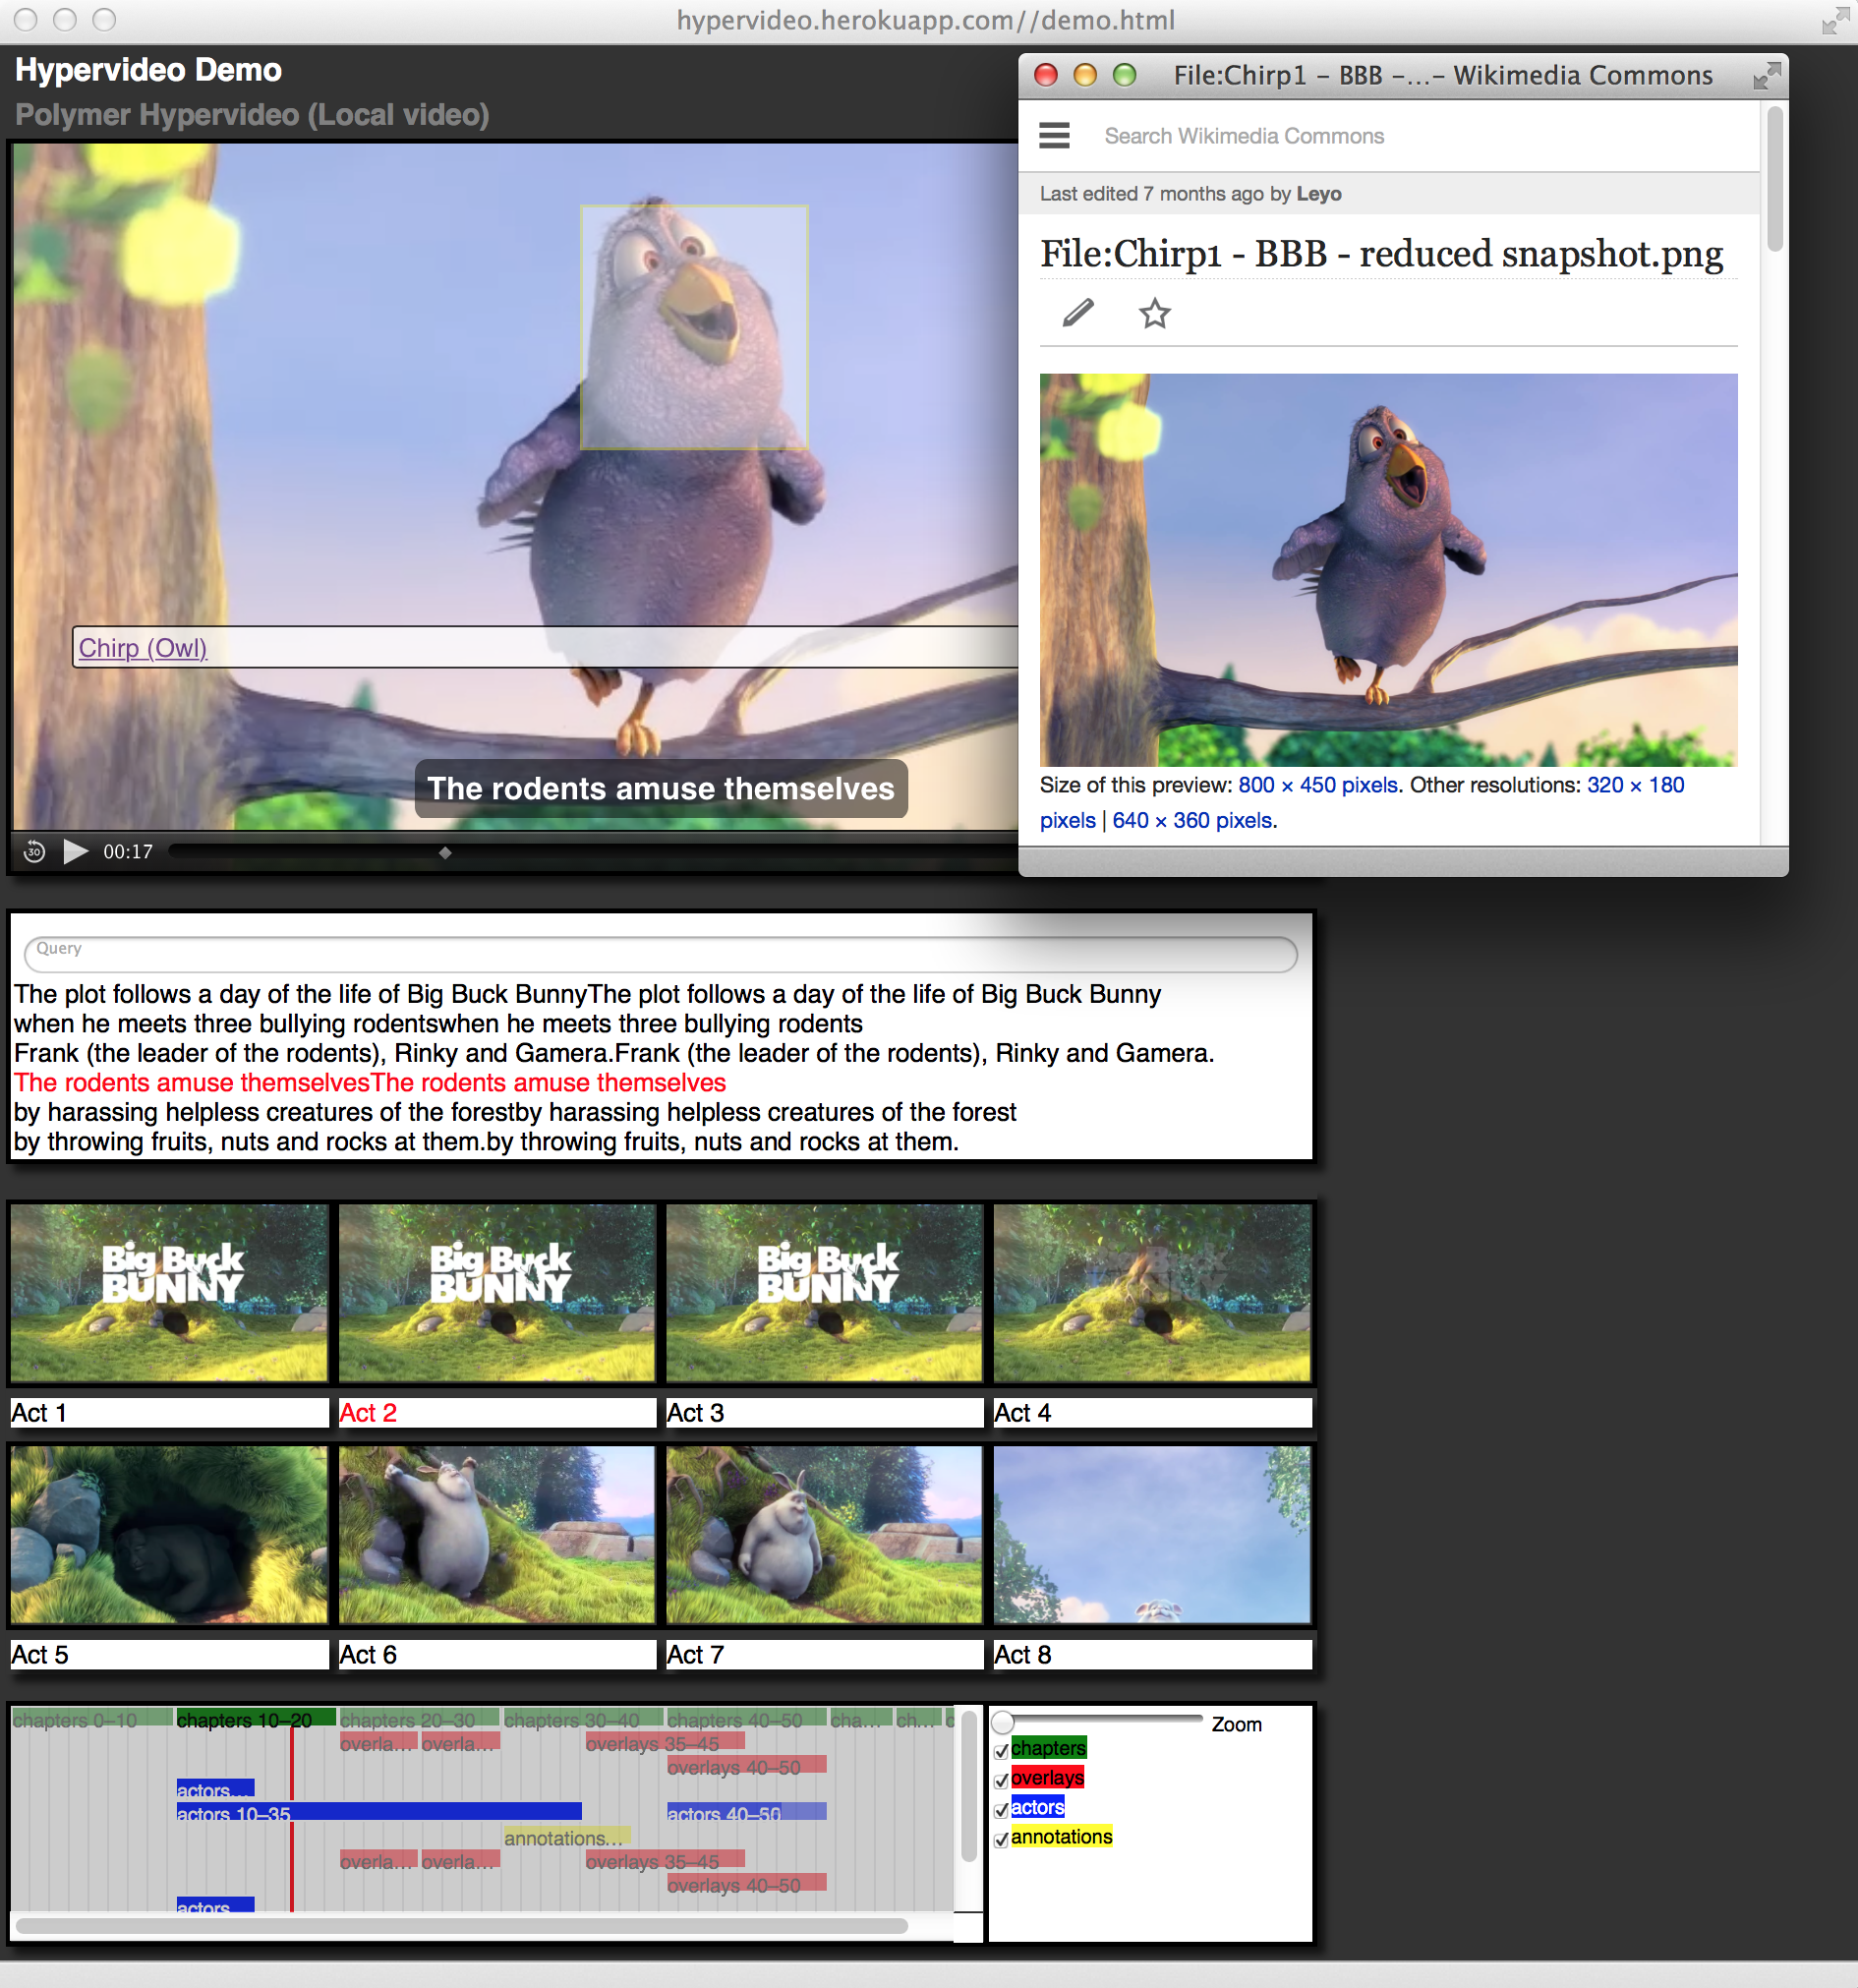
\includegraphics[width=0.39\linewidth]{screenshot}
  \caption{Generated hypervideo based on the mark-up in \autoref{listing:polymer},
  including subtitles, chapters, timeline, and table of contents;
  the actor annotation contains a spatial fragment~\cite{troncy2012mediafragments}
  (owl's head) and a~link
  to a~Wikimedia Commons page}
  \label{fig:screenshot}
\end{figure}

\begin{lstlisting}[caption={Web Components mark-up for the hypervideo in \autoref{fig:screenshot}, including subtitles, chapters, timeline, and table of contents; the actor annotation contains a spatial fragment
(\texttt{xywh})~\cite{troncy2012mediafragments} and a~link (\texttt{url})
  to Wikimedia Commons},
  label=listing:polymer, language=xml,
  float=p!, stringstyle=\color{gray},morekeywords={polymer,hypervideo,track,subtitles,chapters,toc,timeline,visualization,data,actor,src,end,start,name,url,width,height,muted,displaysubtitlesgroup,orientation,displaychaptersthumbnails,xywh}]
<polymer-hypervideo src="big_buck_bunny.mp4 big_buck_bunny.webm" width="400" height="225" muted>
  <polymer-data-actor start="10" end="35" name="Chirp (Owl)" xywh="170,20,70,80" 
      url="http://commons.m.wikimedia.org/wiki/File:Chirp1_-_BBB_-_reduced_snapshot.png">
  </polymer-data-actor>
  <polymer-track-subtitles src="subtitles.vtt" displaysubtitlesgroup></polymer-track-subtitles>
  <polymer-track-chapters src="thumbs.vtt" displaychaptersthumbnails></polymer-track-chapters>
  <polymer-visualization-timeline orientation="landscape"></polymer-visualization-timeline>
  <polymer-visualization-toc></polymer-visualization-toc>
</polymer-hypervideo>
\end{lstlisting}

\begin{lstlisting}[caption={Native JavaScript event communication
  between Web Components},
  label=listing:events, language=JavaScript,
  float=p!, stringstyle=\color{gray},morekeywords={addEventListener,document}]
// === In polymer-hypervideo.js: ===
// listen to native html5 video timeupdate events
video.addEventListener('timeupdate', function() {
  that.currentTime = video.currentTime;
  // publish hypervideotimeupdate events
  that.fire('hypervideotimeupdate', { currentTime: that.currentTime });
});

// === In polymer-visualization-timeline.js: ===
// listen to hypervideotimeupdate events
document.addEventListener('hypervideotimeupdate', function(e) {
  var currentTime = e.detail.currentTime;
  // update the time marker
});
\end{lstlisting}

\section{Linked Data Consumation and Publication}

In this section, we first introduce the concept of Linked Data
and Tim Berners-Lee's Linked Data principles,
and then Ruben Verborgh's Linked Data Fragments.
This leads us to the \emph{Spectacle en Ligne(s)} Linked Data portal,
whose data we consume in our application in an ``eat your own dog food'' manner.

\subsection{Introduction to Linked Data}

Linked Data~\cite{bernerslee2006linkeddata} defines a~set of agreed-on
best practices and principles for interconnecting and publishing structured data on the Web.
It uses Web technologies like the Hypertext Transfer Protocol~\cite{fielding1999http}
and Unique Resource Identifiers (URIs,~\cite{bernerslee2005uri})
to create typed links between different sources.
The portal \url{LinkedData.org} defines Linked Data as being
``about using the Web to connect related data that wasn't previously linked,
or using the Web to lower the barriers to linking data currently linked using other methods.''
Tim Berners-Lee defined the four rules for Linked Data in a~W3C Design Issue as follows:

\begin{enumerate}
	\item Use URIs as names for things.
	\item Use HTTP URIs so that people can look up those names.
	\item When someone looks up a URI, provide useful information, using the standards (RDF, SPARQL).
	\item Include links to other URIs, so that they can discover more things.
\end{enumerate}

Linked Data uses the Resource Description Framework (RDF,~\cite{klyne2004rdf})
to create typed links between things in the world.
The result is often-times referred to as the Web of Data.
RDF encodes statements about things in the form of triples that take the form subject, predicate, object. 
In this context, Heath and Bizer~\cite{bizer2009linkeddatastory} also speak of RDF links,
\emph{i.e.}, dereferencing the URI that appears as the destination of a~link
yields a~description of the linked resource.

\subsection{Linked Data Fragments}
Various access mechanisms to Linked Data exist on the Web,
each of which comes with its own trade-offs regarding query performance, freshness of data,
and server cost/availability.
To retrieve information about a specific subject, you can dereference its URL.
SPARQL~\cite{prudhommeaux2008sparql} endpoints allow to execute complex queries on RDF data,
but they are not always available.
While endpoints are more convenient for clients, individual requests
are considerably more expensive for servers.
Alternatively, a data dump allows interested parties to query locally.
Linked Data Fragments~\cite{verborgh2014ldf} provide a~uniform view
on all such possible interfaces to Linked Data,
by describing each specific type of interface by the kind of fragments through which
it allows access to the dataset.
Each fragment consists of the three following parts:

\begin{description}
	\item[data:] all triples of this dataset that match a specific selector;
	\item[metadata:] triples that describe the dataset and/or the Linked Data Fragment;
	\item[controls:] hypermedia links and/or forms that lead to other Linked Data Fragments.
\end{description}

This view allows to describe new interfaces with different trade-off combinations.
One such interface is triple pattern fragments~\cite{verborgh2014triplepatterns},
which enables users to host Linked Data on low-cost servers with higher availability
than public SPARQL endpoints.
Such a~light-weight mechanism is ideal to expose mid-size datasets on commodity hardware
in a~scalable and ad hoc manner using triple pattern fragments.

\begin{figure}
        \centering
        \begin{subfigure}[b]{\textwidth}
                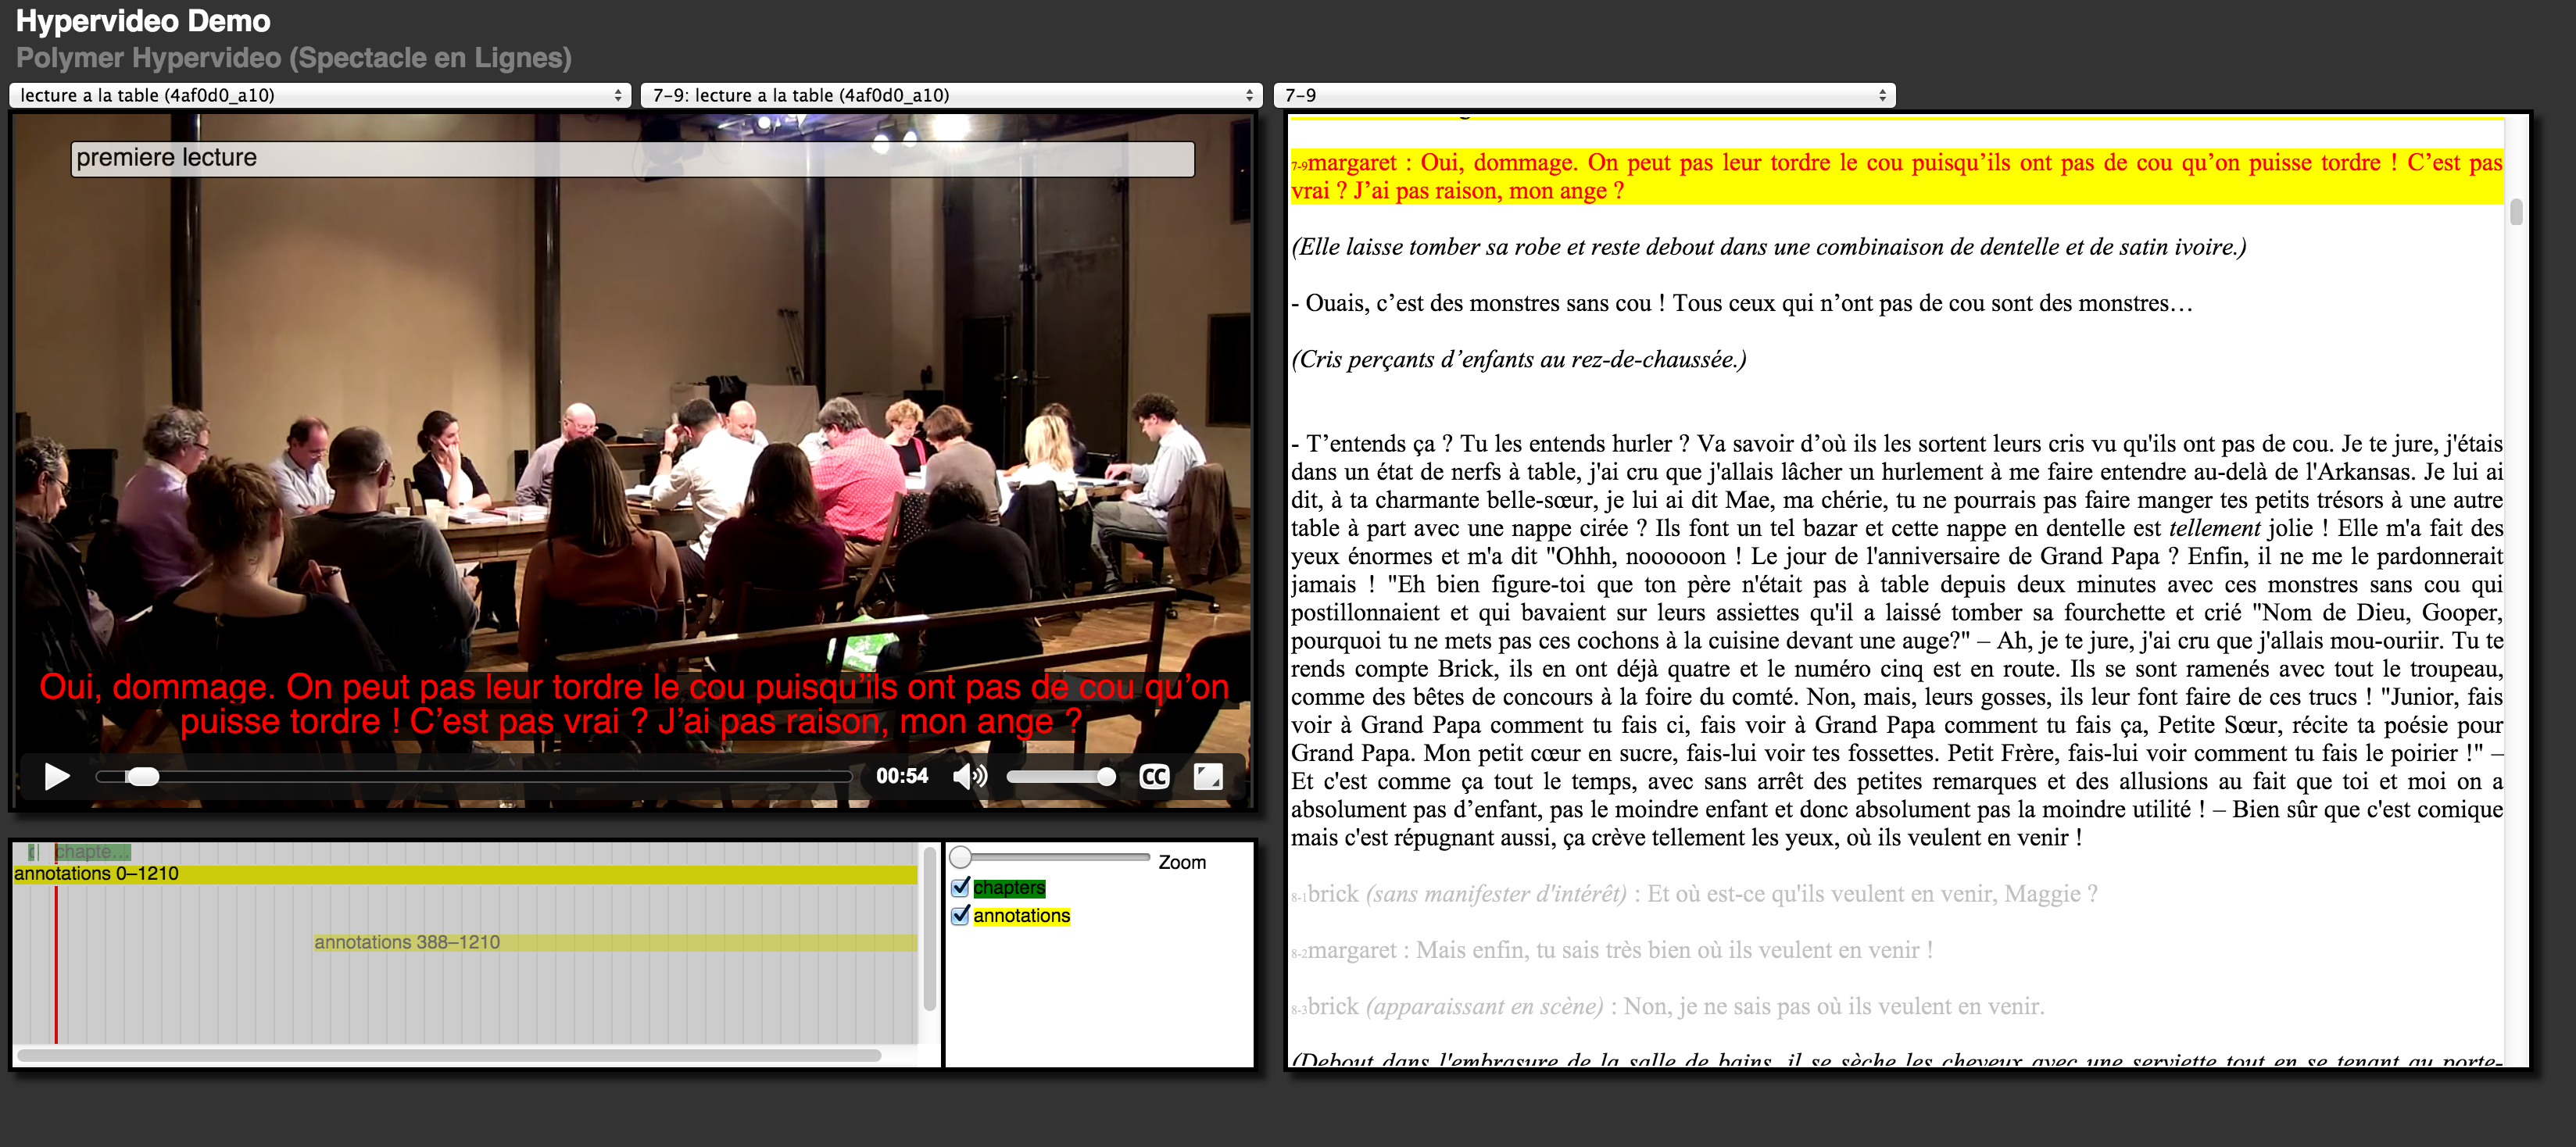
\includegraphics[width=\textwidth]{spel1}
                \caption{Day~1, first lecture at the table,
                	\url{http://spectacleenlignes.fr/hypervideo/\#lecture-a-la-table_4af0d0_a10/7-9}}
                \label{fig:day1}
        \end{subfigure}
        
        \begin{subfigure}[b]{\textwidth}
                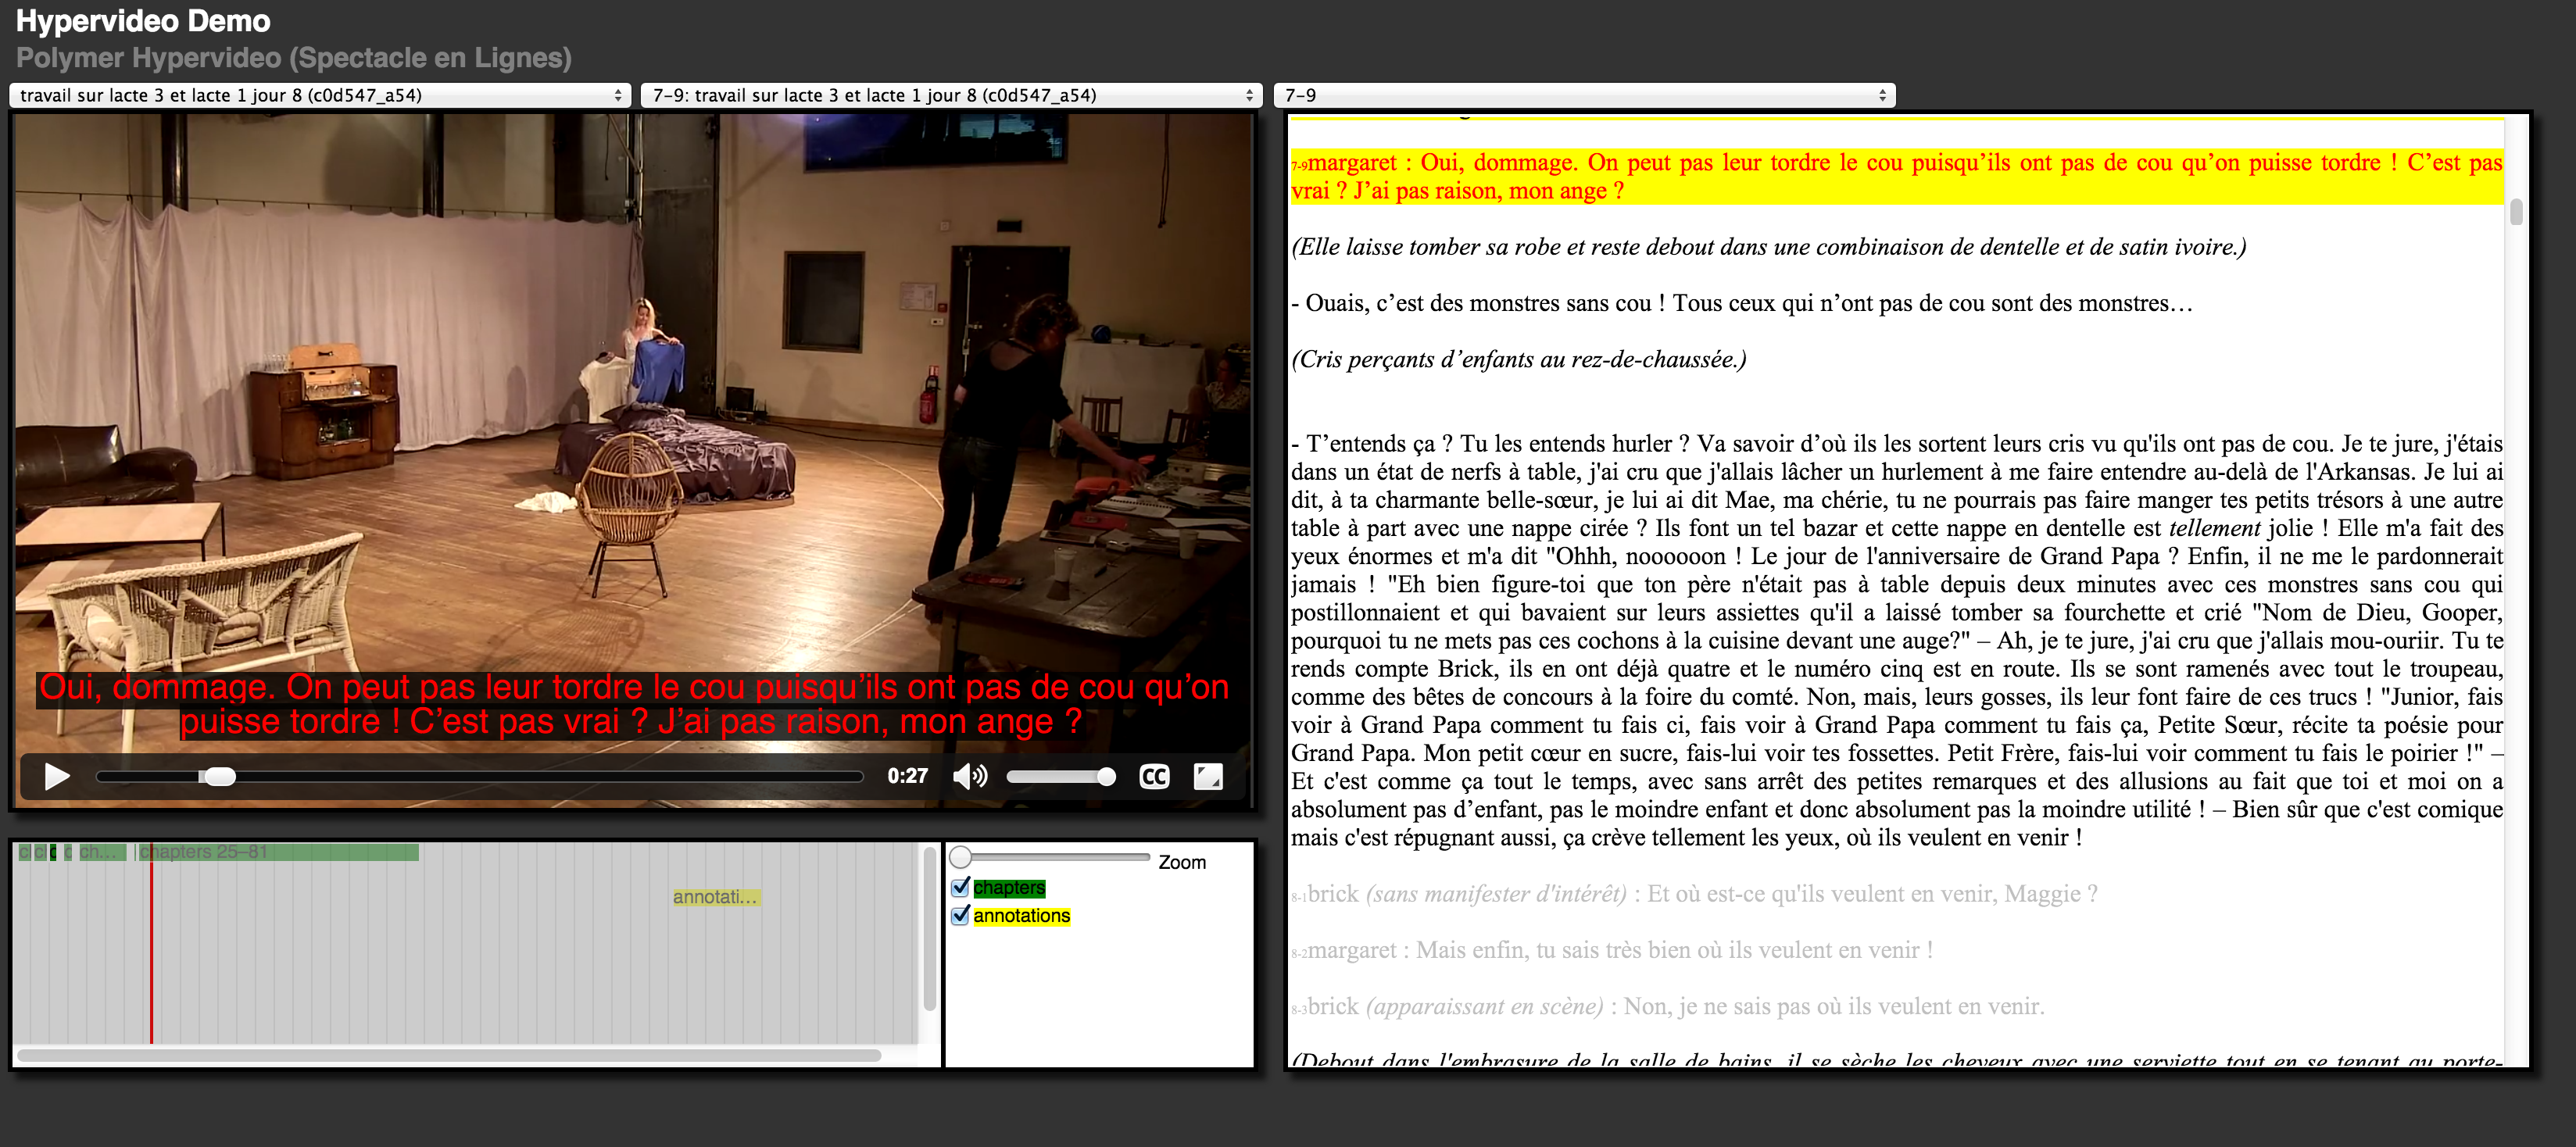
\includegraphics[width=\textwidth]{spel2}
                \caption{Day~8, rehearsals of act~1,
                	\url{http://spectacleenlignes.fr/hypervideo/\#travail-sur-lacte-3-et-lacte-1-jour-8_c0d547_a54/7-9}}
                \label{fig:day8}
        \end{subfigure}
        
        \begin{subfigure}[b]{\textwidth}
                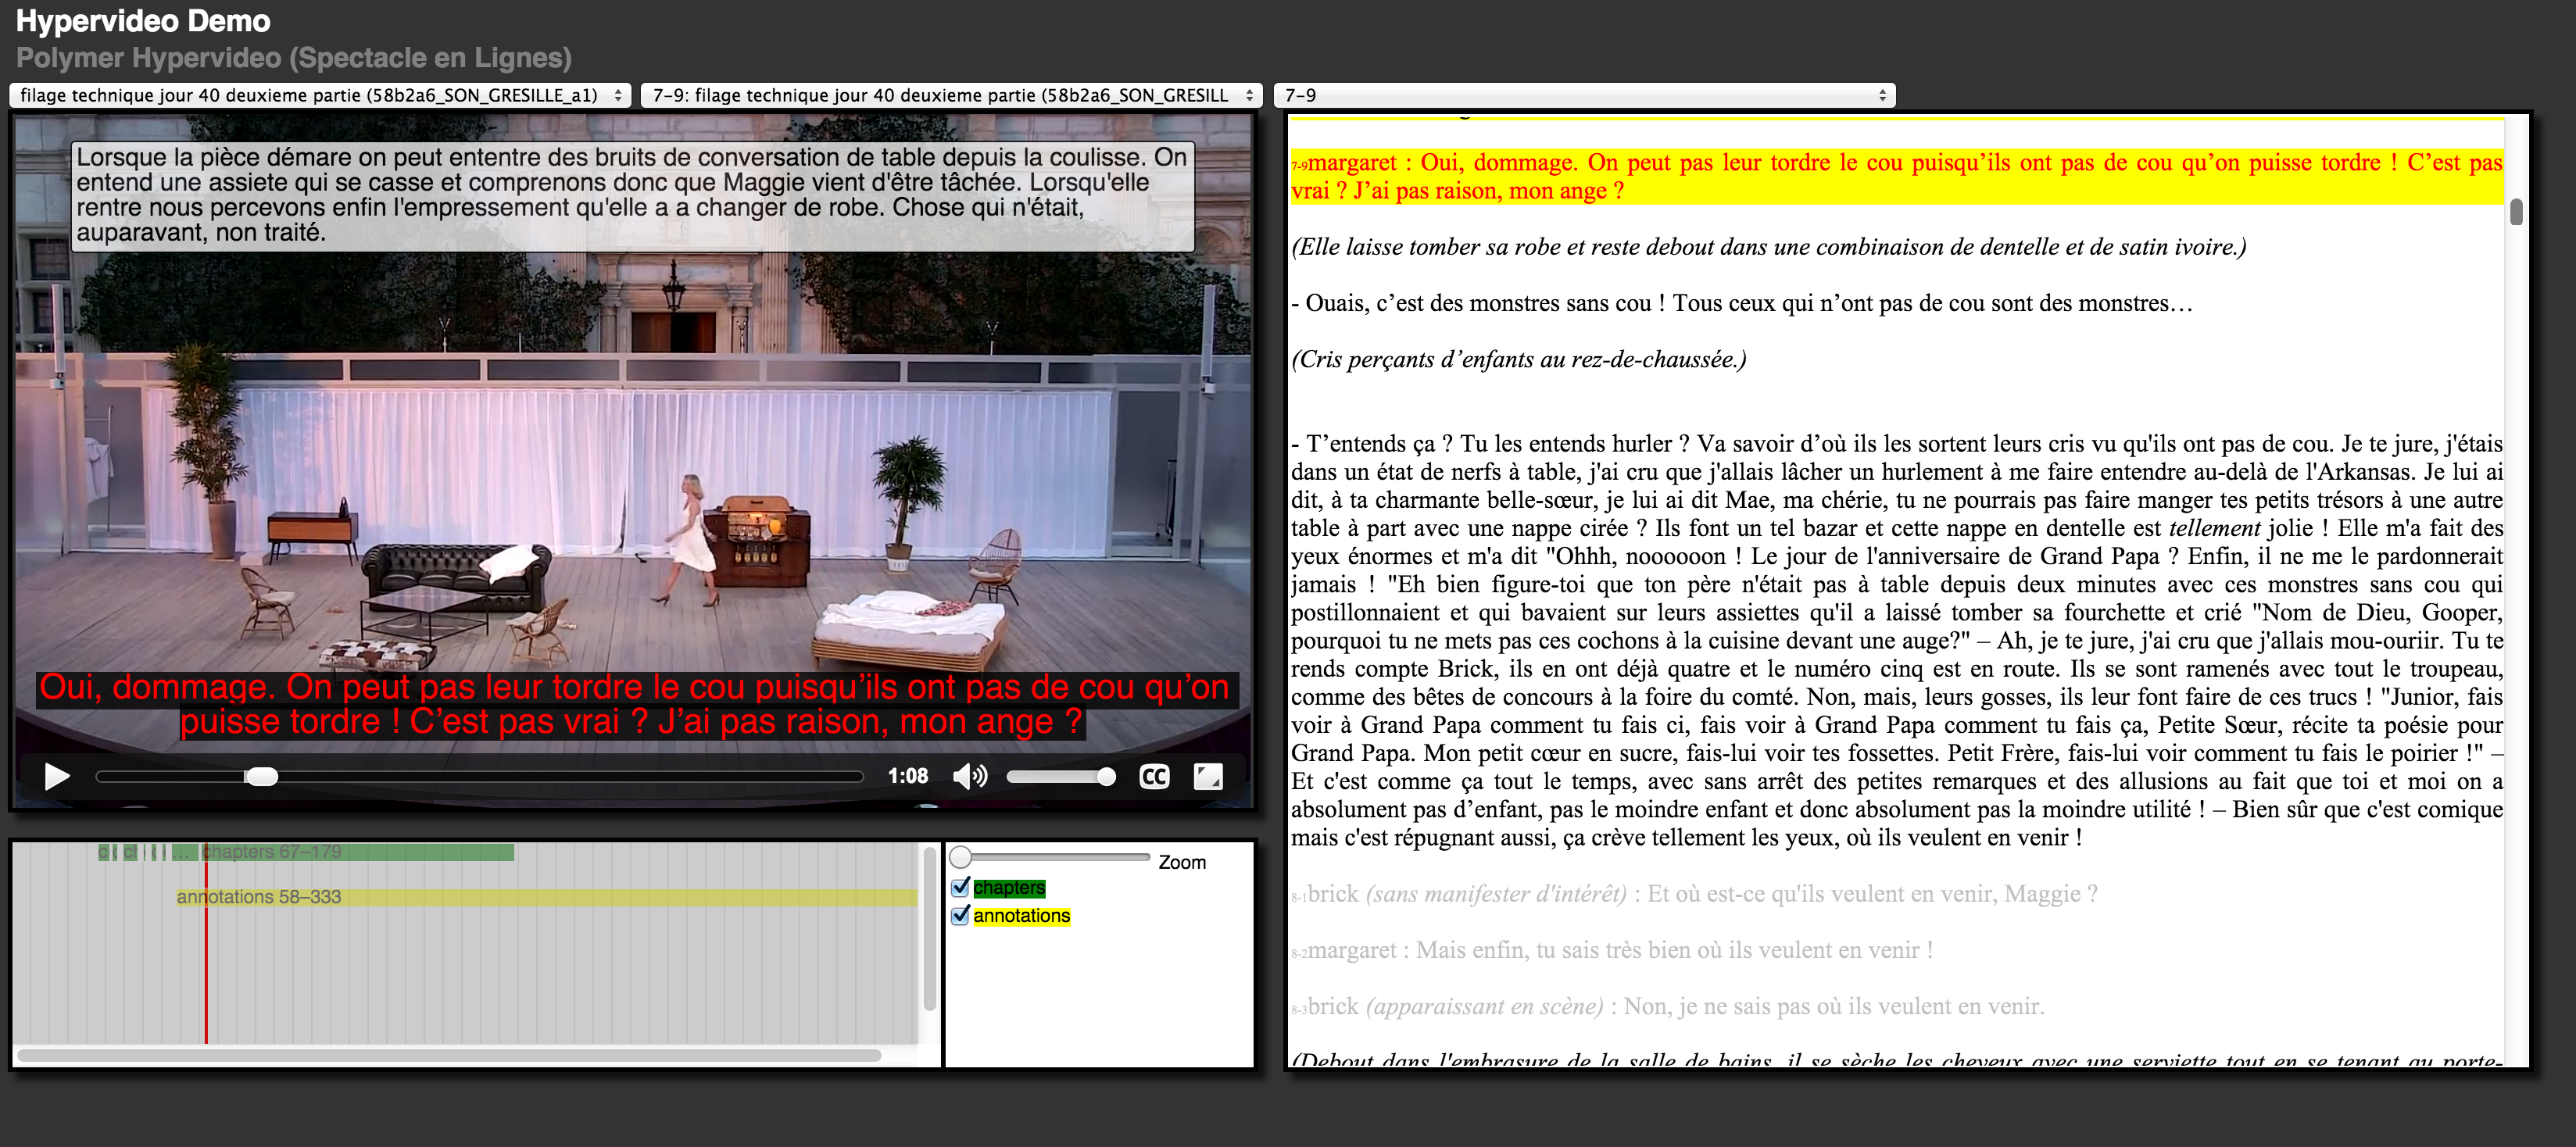
\includegraphics[width=\textwidth]{spel3}
                \caption{Day~40, technical mise en scène,
                	\url{http://spectacleenlignes.fr/hypervideo/\#filage-technique-jour-40-deuxieme-partie_58b2a6_SON_GRESILLE_a1/7-9}}
                \label{fig:day40}
        \end{subfigure}
        \caption{Evolution of act~1, cue 7.9 of T. Williams' \emph{Chatte Sur Un Toit Brulant}}\label{fig:animals}
\end{figure}

\section{Conclusions and Future Work}

In this paper, we have introduced a~Web-Components-based approach
for the generation of hypervideos with nothing more than custom HTML elements.
We have made both a~demo application and the underlying source code
as well as the source code of the mentioned Web Components available.
Immediate next steps are to improve the browser compatibility
and to migrate the code to the native Web Components implementation
that will soon be encountered in all major Web browsers.
Concluding, Web Components radically redefine how we develop applications
on the Web.
With our code, we have shown that this certainly holds true for hypervideo
and are excited about future applications and use cases.

\bibliographystyle{abbrv}
\bibliography{references}
\end{document}
